\section{Versuchsaufbau und Durchführung}
\label{sec:Durchführung}
Zunächst wird der Aufbau des Versuchs beschrieben.
\subsection{Versuchsaufbau}
\label{ssec:Versuchsaufbau}
Der Versuchsaufbau ist in \autoref{fig:aufbau}
\begin{figure}[H]
    \centering
    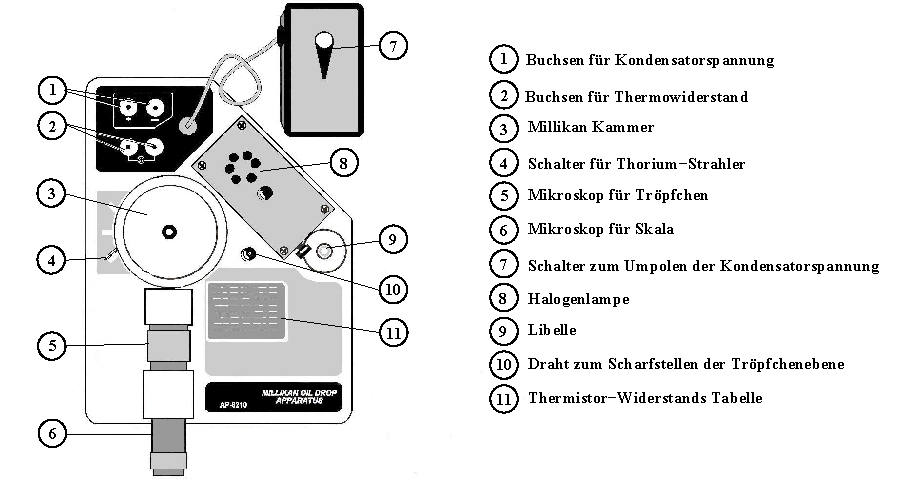
\includegraphics{content/graphics/Aufbau.pdf}
    \caption{Aufbau des Millikan-Versuchs \cite{v503}}
    \label{fig:aufbau}
\end{figure}
dargestellt. Die Tröpfchen gelangen durch den Zerstäuber in die Millikan Kammer.
In dieser gibt es einen Kondensator der ein elektrisches Feld senkrecht zur Bewegungrichtung der Tröpfchen generiert.
Der Kondensator kann ein und aus geschaltet aber auch durch einen Hebel umgepolt werden.
Dies erlaubt es das Elektrische Feld umzukehren und die Tröpfchen in beide Richtungen zu beobachten.
Nicht alle Tröpfchen müssen durch die Reibung in der Zerstäubung aufgeladen worden sein, weshalb ein schwach radioaktives Präparat
in der unteren Platte eingelassen ist. Dieses ist verdeckt und kann durch einen Schalter abgedeckt werden.
Die radioaktive Stahlung des Thorium-232 Präparates ionisiert die Luft in der Kammer und kann so sie
Tröpfchen aufladen. Da die Tröpfchen zu klein sind um genau mit dem Auge beobachtet zu werden wird ein Mikroskop verwendet.
Mithilfe der Längenskala im Hintergund kann so sie Geschwindigkeit der Tröpfchen bestimmt werden.
Um diese gut zu erkennen werden sie mit einer Halogenlampe beleuchtet. Da diese die Luft in der Kammer erwärmt wird die Temperatur durch einen Thermister-Widerstand bestimmt.
Da es in diesem Versuch wichtig ist das die Tröpfchen senkrecht nach unten fallen ist ebenfalls eine Libelle, zum ausrichten der Kammer, angebracht.
\subsection{Durchführung}
\label{ssec:Durchführung}
Nach korrektem Ausrichten der Kammer mithilfe der Libelle wird ein wenig Öl in die Kammer gestäubt.
Es sollte allerdings nicht zu viel Öl in die Kammer gegeben werden da die Tröpfchen so nicht mehr gut zu verfolgen sind und etwa fünf Minuten gewartet werden muss bis das Öl am Boden der Kammer ankommt.
Durch das Mikroskop wird ein Tröpfchen das etwa die Geschwindigkeit $v_0=\qty{0.01}{\meter\per\second}$ bis $v_0=\qty{0.001}{\meter\per\second}$ bestitzt gesucht.
Nun wird der Kondensator mit Spannung versorgt und das Tröpfchen beobachtet sollte sich die Bewegung nicht ändern wird der Kondensator abgeschaltet
und mit dem Thorium-232 Päparat das Tröpfchen geladen.
Wenn der Kondensator nun wieder eingeschaltet wird erfährt dieses eine Kraft und es wird die neue Geschwindigkeit $v_{ab}$ bzw. $v_{auf}$ bestimmt.
Hierzu wird die Zeit die für einen bestimmten Weg benötigt wird gemessen. Mit der umgekehrten Polung am Kondensator wird so auch die andere Geschwindigkeit gemessen.
Wichtig ist das nur Tröpfchen beachtet werden für die gilt $2v_0=v_{ab}-v_{auf}$. Wenn dies nicht der Fall ist hat sich die Ladung während der Messung geändert.
Die so berechnete Ladung ist also nicht brauchbar.
Diese Messungen werden für fünf Tröpfchen drei mal wiederholt, wobei $v_0$ nur einmal bestimmt wird. Dann wird die Kondensatorspannung erhöht.
Bei dieser werden fünf weitere Tröpfchen gemessen. Die Kondensatorspannung sollte dabei nicht über $\qty{500}{\volt}$ betragen.
Wichtig ist es zudem etwa alle 15 Minuten die Temperatur zu bestimmen, um mit dieser die Viskosität von Luft aus \autoref{fig:visko} abzulesen.
\begin{figure}[H]
    \centering
    \includegraphics{content/graphics/Viskosität.pdf}
    \caption{Viskosität von Luft bei verschiedenen Temperaturen \cite{v503}}
    \label{fig:visko}
\end{figure}
Der Thermistor-Widerstand gibt allerdings nur Widerstände aus weshalb mit Hilfe von \autoref{fig:temp} die Temperatur bestimmt wird.
\begin{figure}[H]
    \centering
    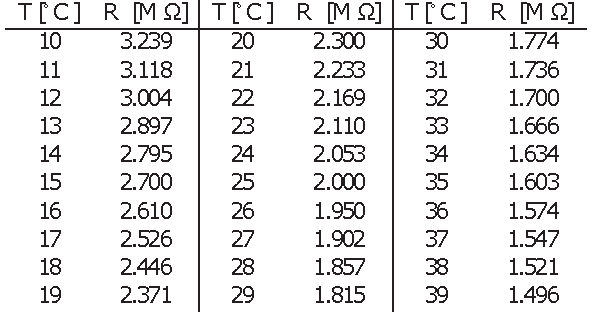
\includegraphics{content/graphics/Temperatur.pdf}
    \caption{Temperatur der Luft bei verschiedenen Widerständen \cite{v503}}
    \label{fig:temp}
\end{figure}
Durch diese Messungen lässt sich die Elementarladung bestimmen.
